\section{Architecture}

%insert image of the system architecture
\begin{figure}[h]
	\centering
	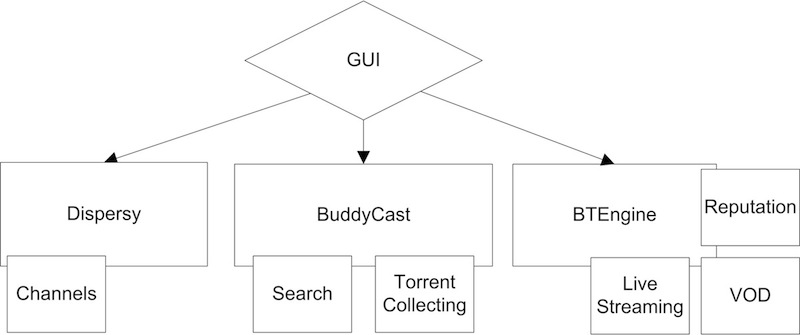
\includegraphics[scale=0.4]{tribler/images/tribler_component_overview.jpg}
	\caption{The architecture of Tribler}
	\label{fig:tribler_components}
\end{figure}

Tribler consists out of four major components as can also be seen in figure \ref{fig:tribler_components}\footnote {http://sigmm.org/records/records1201/featured03.html}:
\begin{itemize}
	\item GUI: the graphical user interface.
	\item BTengine: the bittorrent engine.
	\item BuddyCast: a protocol for communication between peers
	\item Dispersy: a protocol similar in function to BuddyCast, but scalable.
\end{itemize}

\subsection{GUI}

\subsection{Bittorrent}

\subsection{P2P communication}



Tribler: A social-based Peer-to-Peer system paper
https://github.com/Tribler/tribler/wiki
http://iptps06.cs.ucsb.edu/papers/Pouw-Tribler06.pdf